\documentclass[output=paper]{LSP/langsci} 
\ChapterDOI{10.5281/zenodo.1090986}
\title{``All I know is that I know nothing''? Empirical evidence of self-confidence and inexperience in novice vs. professional translators}
\author{Carla Quinci}
\affiliation{Università di Trieste}

\abstract{In the last few decades, translation competence (TC) has been largely investigated but ``most of the proposals concerning TC have not been empirically tested and only a few of them have attempted to validate their models from an empirical-experimental perspective'' \citep[64]{Hurtado2009}. Drawing on this, an empirical longitudinal study has been designed to investigate whether TC can be defined in terms of specific textual and procedural patterns shared by professional translators and observe whether such trends are being developed by trainee translators throughout their training. The investigation mainly relies on the contrastive analysis of multiple translations of the same six source texts produced at regular intervals over three years (2012-2014) by translators at different stages in the development of their TC and considers a variety of textual and procedural features in the attempt to identify possible patterns in the groups of participants. This paper focuses on some process-related results providing evidence of unawareness and self-confidence in novice vs. more experienced trainees and professional translators.}
\shorttitlerunninghead{``All I know is that I know nothing?''}
\maketitle
\begin{document}

\section{Introduction}

Any learning process implies a progress from (relative) ignorance to the acquisition of knowledge. Any learner should thus be aware of being somehow lacking and in search of something she does not possess. This awareness can be considered the driving force behind the learning process, allowing the learner to recognise and ultimately reach the final goal of her path. However, such consciousness is often gained through learning and experience since it is acquired knowledge itself that opens up new horizons in the learner's mind, making her aware of knowledge yet to be attained.

Empirical research in Translation Studies suggests that ``\isi{novices} are blissfully unaware of their ignorance'' \citep[67]{Jaaskelainen1996} and tend to be more self-confident than their actual competence would justify. This paper will provide further insights into unawareness and self-confidence in novice vs. professional translators obtained through a longitudinal empirical study on \isi{translation competence} (TC) and its development.

\section{Preliminary theoretical remarks}

Research on TC has been quite productive in the last few decades, devising a wide variety of possible definitions and models for both didactic and professional purposes. Still, despite the ever-increasing efforts put into the empirical analysis of TC and its development, little consensus has been reached in academia on the nature and modelling of such competence.

TC is generally assumed to be ``qualitatively different from bilingual competence'' (\citealt[44--45]{PACTE2002}; cf. \citealt{Lorscher2012}) and non-innate \citep[121]{Shreve1997} since a ``basic translation ability is a necessary condition, but no guarantee, for further development of a (professional) competence as a translator, and possibly expertise in translation'' \citep[12]{Englund2005}. Except for these two widely agreed-upon assumptions, a considerable number of concurrent terms and conceptual frameworks have been devised in the attempt to identify the essential constitutive components of TC (for an overview, cf. \citealt{Orozco2002}; \citealt{Quinci2015a}). Most recent approaches tend to opt for a multicomponential conceptualisation of TC, which would be made up of a varying number of different or (partially) overlapping sub-competences that are generally deemed to be interdependent and interacting with one another. Recently, these have also been represented as individual vortices gradually merging in the larger vortex of translation supercompetence, in which the unpredictable number and types of linkages between the different sub-components increases with training and experience \citep{Kiraly2013}.

Although empirical research on TC has still a long way to go, from the mid-1980s onwards, empirical studies have considerably contributed to the investigation of TC and have, in some cases, resulted in the development of empirically validated definitions and models \citep{Gopferich2009Towards, PACTE2003}. Most empirical evidence, however, relate to the \isi{translation process}, i.e. to the analysis of behavioural and procedural features of (un)experienced translators, so as to identify possible common patterns which might be conductive to high (or poor) \isi{translation quality}. To provide a complementary perspective to such mainstream methodology, an empirical longitudinal study has been designed adopting a combined approach, which is mainly product-oriented but also encompasses process-related data. Partial results from the aforementioned research project will be presented in the following sections, suggesting a higher degree of self-confidence and unawareness in \isi{novices} as compared to (more) experienced translators.\footnote{At the time of writing the PhD research project was still ongoing. Its final results and conclusions are now available \citep{Quinci2015b} and can be accessed at \url{http://hdl.handle.net/10077/10986}.}

Self-awareness and self-confidence are ``two psychological features which are part of the make-up of a \isi{professional translator}'' \citep[32]{Kussmaul1995Training}, with self-aware\-ness (or self-concept) being often implicitly or explicitly included in most recent models of TC (\citealt{Gopferich2009Towards}; \citealt{Kiraly1995Pathways}; \citealt[93]{PACTE2003}). The two concepts are in fact ``closely linked [as it] is through self-awareness that translators gain self-confidence'' \citep[32]{Kussmaul1995Training} and ultimately ``visualize themselves as text designers than as text reproducers'' \citep[34]{Gopferich2009Towards}. Although these two psychological features should ideally be developed through specific training \citep[34]{Gopferich2009Towards}, it has been observed that when ``students embark on a translator training course, they are quite self-confident young people, but in the course of their studies they lose their self-confidence as a result of the criticism of their teachers'' \citep[32]{Kussmaul1995Training}. This is in line with the results of this study, showing an unjustified higher level of self-confidence in novice translators (which is not supported by equally high-quality outcomes) which gradually decreases throughout their training. However, this is not necessarily due to teachers' criticism, but may also result from a growing ability to assess \isi{translation quality} and identify translation errors and problems, which is progressively developed throughout the training programme.

\section{Research design and methodology}

Given its longitudinal design, the study included six translation tasks which have been performed at regular intervals over a three-year period, so as to analyse from a synchronic perspective the discrepancies and similarities in the performances of translators with different levels of TC and \isi{monitor} diachronically the evolution of such patterns in the same groups of participants. The 63 voluntary participants at different stages in the development of their TC included BA, first- and second-year MA translation trainees and professional translators, falling into four distinct groups, i.e. Group N (`\isi{novices}'), Group I\textsubscript{1} and Group I\textsubscript{2} (first- and second-year `intermediates'), and Group P (`professionals') respectively. The internal composition of the four groups has remained almost completely unchanged throughout the duration of the study, even though the cohorts included in the groups of intermediates (i.e., Ia, Ib, Ic, and Id) have varied during the investigation alongside students' progress in their training programme, as shown in \tabref{quinci:tab:1} below.

\begin{table}
\footnotesize
\caption{Internal composition of the sample}
\label{quinci:tab:1}
\begin{tabularx}{\textwidth}{>{\raggedright}XXXX}
\lsptoprule
 & \multicolumn{3}{c}{Academic Year}\\\cmidrule(lr){2-4}
 & \multicolumn{1}{c}{2011/12} & \multicolumn{1}{c}{2012/13} & \multicolumn{1}{c}{2013/14}\\\midrule
 BA Students (Novices) & GROUP N:\par 13 1\textsuperscript{st}-year students & GROUP N:\par 13 2\textsuperscript{nd}-year students & GROUP N:\par 13 3\textsuperscript{rd}-year students\\
 1\textsuperscript{st} year MA Students (Intermediates) &  GROUP I\textsubscript{1} (Ia):\par 7 1\textsuperscript{st}-year students & GROUP I\textsubscript{1} (Ic):\par 10 1\textsuperscript{st}-year students &  GROUP I\textsubscript{1} (Id):\par 12 1\textsuperscript{st}-year students\\
 2\textsuperscript{nd} year MA Students (Intermediates) & GROUP I\textsubscript{2} (Ib):\par 10 2\textsuperscript{nd}-year students & GROUP I\textsubscript{2} (Ia):\par 7 2\textsuperscript{nd}-year students & GROUP I\textsubscript{2} (Ic):\par 9 2\textsuperscript{nd}-year students\\
 Professionals & GROUP P:\par 9 participants & GROUP P:\par 9 then 8 participants & GROUP P:\par 8 participants\\
 Partic. per year & 39 & 39 then 38 & 42\\
 \lspbottomrule
\end{tabularx}
\end{table}

\largerpage
The tasks were specifically designed to gather both product- and process-re\-lat\-ed data and involved the translation of six non-specialist articles from English into \ili{Italian}, the participants' mother tongue, as well as a post-task questionnaire investigating the \isi{translation process}. Despite the study's primarily product-oriented approach involving twelve different variables (e.g. expansions and reductions, lexicometric measures, lexical density and variation, vocabulary analysis), this paper only focuses on some process-related data highlighting \isi{novices}' self-confidence and unawareness, which are then contrasted with data on translation \isi{acceptability}. Given its primary orientation towards product analysis, the study did not resort to think-aloud protocols (TAPs), screen activity recordings or other methods generally used for gathering process data, but only to a post-task questionnaire regarding different process-related issues, e.g. the first reading and the perceived level of difficulty of the ST, the \isi{revision} process, the reference materials used, other training and working activities which could affect the development of TC.

The analysis outlined in the following sections integrates data concerning the use of reference materials, \isi{revision} and \isi{acceptability} into existing provisional results relating to delivery time, self-assessment and perceived text difficulty, which in this case also include new data from the fifth translation task. After a brief overview of previous results \citep{Quinci2015a}, the analysis focuses on data about the use of reference materials and \isi{revision} and finally relates all the above process-related data with the evaluation of translation \isi{acceptability}, so as to point out the procedural features shared by all good-performing participants.

For a more reader-friendly representation of the patterns identified, the tables below simultaneously show the groups' scores and ranking by means of conditional formatting using a colour scale from red to green to differentiate high, middle, and low values respectively. Finally, the thicker lines in the tables divide the tasks performed in the same academic year (and thus by the same cohorts of participants), i.e. 2011/2012 for tasks 1 and 2, 2012/2013 for tasks 3 and 4, and 2013/2014 for task 5.

\section{Previous results: A follow-up}

First results from the joint analysis of participants' delivery time, self-assessment and perceived text difficulty scores showed a high level of self-confidence in novice translators. In particular, \isi{novices} generally recorded comparatively low delivery time and high self-assessment scores which appear not to result from underestimating the task difficulty, but rather from overestimating their translation abilities and probably from their limited ability to assess \isi{translation quality}.

\begin{table}
\caption{Average delivery time per group and task}
\label{quinci:tab:2}
\begin{tabular}{lrrrr}
\lsptoprule
& N & I\textsubscript{1} & I\textsubscript{2} & P \\
\midrule
T1 & 01:26 & 01:47 & 01:39 & 01:25\\
T2 & 01:30 & 01:34 & 01:42 & 01:07\\
T3 & 01:28 & 01:43 & 01:28 & 01:00\\
T4 & 01:26 & 01:35 & 01:33 & 01:13\\
T5 & 01:29 & 01:33 & 01:36 & 01:14\\
\midrule
mean & 01:28 & 01:39 & 01:36 & 01:12\\
\lspbottomrule
\end{tabular}
\end{table}

\begin{table}
\caption{Average self-assessment scores on a scale from 1 to 10}
\label{quinci:tab:3}
\begin{tabular}{lrrrr}
\lsptoprule
& N & I\textsubscript{1} & I\textsubscript{2} & P\\
\midrule
T1 & 7.4 & 6.9 & 7.0 & 7.2\\
T2 & 7.1 & 6.8 & 6.7 & 7.5\\
T3 & 7.4 & 7.1 & 6.7 & 7.5\\
T4 & 7.2 & 7.0 & 6.7 & 7.1\\
T5 & 7.2 & 7.0 & 6.8 & 7.3\\
\midrule
mean & 7.26 & 6.96 & 6.78 & 7.32\\
\lspbottomrule
\end{tabular}
\end{table}

\begin{table}
\caption{Average perceived text difficulty on a scale from 1 (very easy) to 5 (very difficult)}
\label{quinci:tab:4}
\begin{tabular}{lrrrr}
\lsptoprule
& N & I\textsubscript{1} & I\textsubscript{2} & P \\
\midrule
T1 & 2.53 & 2.85 & 2.70 & 2.66\\
T2 & 3.23 & 3.14 & 3.10 & 2.66\\
T3 & 2.76 & 2.90 & 2.85 & 2.66\\
T4 & 3.00 & 3.00 & 3.00 & 2.87\\
T5 & 3.15 & 2.75 & 2.78 & 3.25\\
\midrule
mean & 2.93 & 2.92 & 2.88 & 2.82\\
\lspbottomrule
\end{tabular}
\end{table}

As concerns the average delivery time, professionals show the highest rates, followed by \isi{novices} who consistently performed faster than both groups of intermediates (\tabref{quinci:tab:2}). Likewise, \isi{novices} and professionals display similar patterns in self-assessment (\tabref{quinci:tab:3}), where they alternatively recorded the highest scores in the five translation tasks. Self-assessment also shows an interesting pattern as concerns the two groups of intermediates, who consistently ranked in the same order as their supposed level of competence, with first-year MA students preceding second-year trainees in all tasks except for task 1. This would suggest a sort of interdependency between the development of TC and the self-\isi{perception} of the quality of the performance. Such relation could be described as a parabola opening upwards, as shown in \figref{quinci:fig:1} below.

\begin{figure}
 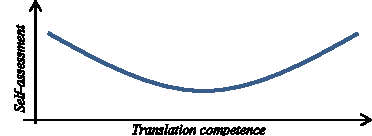
\includegraphics[width=\textwidth]{figures/quinci/figure1.pdf}
 \caption{Relation between self-assessment scores and the development of translation competence}
 \label{quinci:fig:1}
\end{figure}

Higher scores in self-assessment are recorded by both the least and most experienced participants, i.e. \isi{novices} and professionals. On the other hand, intermediates, who are (supposed to be) halfway through the development of TC, tend to record consistently lower self-assessment scores as compared to \isi{novices} despite their longer experience and advanced training in translation. One of the possible reasons for this trend might be sought in the lack of awareness of the actual level of difficulty of the task at hand in novice translators as compared to intermediates. Empirical data however do not seem to support this hypothesis.

As summarised in \tabref{quinci:tab:4} above, \isi{novices} did not in fact perceive the task as less difficult as compared to the other groups, given that they scored highest in two tasks out of five and their ranking considerably varied from one task to another. Also, self-assessment scores and the average perceived text difficulty appear to be mostly in inverse proportion, which means that the highest self-assessment scores of each group mostly correspond to the tasks perceived as the simplest, and vice versa. This implies that all groups of participants are somehow able to evaluate the difficulty of given tasks and tend to rank them accordingly.

Hence, given that \isi{novices}' comparatively high self-assessment scores cannot be ascribed to their inability to evaluate the level of difficulty of the translation task, the trends observed might more probably result from the overestimation of their abilities as translators or their limited ability of assessing \isi{translation quality} -- or ultimately from a combination of both.

The hypothesis of a limited ability to assess \isi{translation quality} appears to be further supported by the correlation between self-assessment scores and the stage of development of TC outlined above. MA-level trainees' lower scores in self-assessment might indeed suggest an increased awareness of and/or ability in evaluating \isi{translation quality} which could result from their advanced theoretical and practical training in translation. Obviously, this assumption needs further confirmation found in the assessment of translation \isi{acceptability}, the results of which are illustrated in a later section.

\section{Other clues from process-related data: Reference material and revision}

\subsection{The use of reference material}

The analysis of other process-related data elicited from the questionnaires has highlighted other patterns concerning the supposed level of TC of the different groups of translators. In particular, as concerns information literacy, participants were asked to specify the number and type of different reference materials used selecting one or more options among those included in the relevant multiple-choice question, i.e. bi- and monolingual paper/on-line/off-line dictionaries, glossaries, on-line general search engines and other possible reference materials to be specified.

From a mere quantitative perspective, i.e. considering the number of different resource materials used in each task (\tabref{quinci:tab:5}), professionals generally relied on a more restricted variety of reference materials, in contrast with Künzli's oberservations (\citeyear{Kunzli2001}:513). Also, they mainly used mono- and bilingual dictionaries, as opposed to students who also heavily relied on on-line search engines to look for parallel texts or occurrences.

\begin{table}
\caption{Average number of different reference materials used}
\label{quinci:tab:5}
\begin{tabular}{lrrrr}
\lsptoprule
& N & I\textsubscript{1} & I\textsubscript{2} & P \\
\midrule
T1 & 2.25 & 3.14 & 2.80 & 2.22\\
T2 & 2.15 & 2.71 & 2.60 & 2.44\\
T3 & 2.77 & 2.60 & 2.71 & 1.89\\
T4 & 2.85 & 2.86 & 2.90 & 2.38\\
T5 & 2.92 & 2.75 & 2.44 & 2.38\\
\midrule
mean & 2.59 & 2.81 & 2.69 & 2.26\\
\lspbottomrule
\end{tabular}
\end{table}

From a qualitative point of view, i.e. when considering the types of reference materials used, the analysis shows that bilingual dictionaries were used by 75-100\% and are therefore the preferred type of reference materials, which would also confirm the findings of earlier TAP studies observing the frequency of use of bilingual dictionaries by (non) professional translators \citep{Jensen1999, Krings1986Was, Kunzli2001}. The second most commonly used reference materials are general-purpose search engines, followed by monolingual dictionaries which hold the third and final position in the ranking being used on average by approximately 54\% of \isi{novices} and professionals and by nearly 69\% of intermediates.

% TODO: figures side by side??
% \begin{multicol}{2}
\begin{figure}
 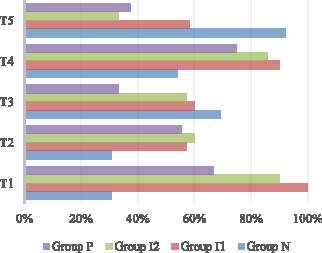
\includegraphics[width=.4\textwidth]{figures/quinci/figure2.pdf}
 \caption{Percentage of participants per group using monolingual dictionaries}
 \label{quinci:fig:2}
\end{figure}

\begin{figure}
 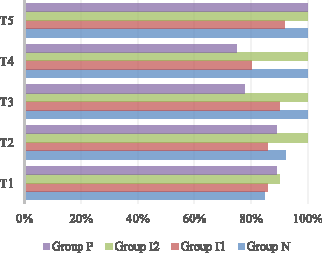
\includegraphics[width=.4\textwidth]{figures/quinci/figure3.pdf}
 \caption{Percentage of participants per group using bilingual dictionaries}
 \label{quinci:fig:3}
\end{figure}
% \end{multicols}

The data on the type reference materials used confirm the trends observed in the quantitative analysis, with professionals mostly ranking in the lower positions and thus referring to a lesser extent to either type of dictionaries. As concerns bilingual dictionaries, a higher average percentage of translation trainees -- both \isi{novices} and intermediates -- resorted to bilingual dictionaries as compared to professionals.

\largerpage
Novices, on the other hand, ranked lowest in three out of five tasks as concerns the use of monolingual dictionaries, which are mostly used by intermediates and professionals. This appears to confirm the results from previous research where more experienced translator ``showed a greater preference for monolingual print and CD/DVD dictionaries than the students did (5th vs. 9th rank)'' (\citealt[197--198]{Massey2011}; cf. \citealt[590]{Ronowicz2005}), although contrary evidence has also been found by \citet[513--514]{Kunzli2001}.

Finally, data also suggest the existence of another pattern of association between age/competence/experience and the use of general Internet search engines, which seems more common among \isi{novices} as compared to professionals, who consistently rank last (\figref{quinci:fig:4}).

\begin{figure}
 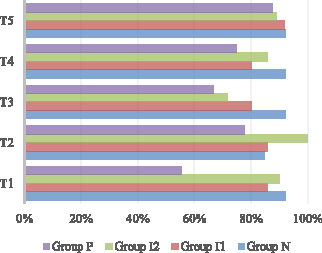
\includegraphics[width=.4\textwidth]{figures/quinci/figure4.pdf}
 \caption{Percentage of participants per group using general search engines}
 \label{quinci:fig:4}
\end{figure}

This would support the claim that ``age is related to the use of Internet resources [as] younger cohorts of translators (i.e. those under 50 years old) are more likely to say that they often or very often use search engines, online multilingual dictionaries, online encyclopedias, and terminology databases to solve linguistic problems than older translators do'' \citep[201]{Massey2011}. However, it should be pointed out that the professional translators in Group P had on average an age of 44, with only one of them older than 50 when entering the sample. Nonetheless, a relation between age and the use of online search engines seems to exist, although it could be equally attributed to the participants' age or their level of TC for lack of direct evidence: trainees, in other words, might be compensating for the lack of information with an increased used of search engines.

It should also be noticed that professionals' low rankings in the use of almost all reference materials (see Figures \ref{quinci:fig:2}, \ref{quinci:fig:3} and \ref{quinci:fig:4}) might in this case be related to their more restricted use of reference materials in general (\tabref{quinci:tab:5}). Other studies on the number of dictionary look-ups have indeed observed ``a reduction in the number of dictionary searches as a function of expertise'' (\citealt[200]{Lesznyak2008}; cf. \citealt[113]{Jensen1999}; \citealt[588]{Ronowicz2005}). Such limited use of reference materials, in terms of both variety and frequency, might result from professionals' deeper knowledge of both the source and \isi{target language}, or better from what Bell defined as ``Frequent Lexis Store'' (FLS), viz. the ``mental (psycholinguistic) correlate to the physical \textit{glossary} or \textit{terminology database}, i.e., an instant `look-up' facility for lexical items both `words' and `idioms''' (1991:47, original emphasis). As pointed out by \citet[583]{Ronowicz2005}, ``[o]ne would [\ldots] expect that more experienced translators will have a larger and more diversified FSS [Frequent Structures Store] and FLS, which should influence the speed and quality of their performance'' -- and ultimately forster the development of justified self-confidence and self-awareness. This hypothesis would be indeed supported by the higher frequency of dictionary searches in \isi{novices} observed in the abovementioned TAP studies, as suggested by \citet[589]{Ronowicz2005}, as well as by the above results concerning the different reference materials used and the participants' delivery time, where professionals consistently performed faster than the other groups.

\subsection{Revision and supposed level of translation competence}

As concerns the \isi{revision} of the target texts (TTs) produced within the study, participants were asked to indicate whether they had self-revised their translations or not and, if yes, whether they carried out ``unilingual'' and/or ``comparative re-reading'' \citep[App. 5]{Mossop2014Revising3rd}, i.e. whether they checked their translations by reading only their TTs (unless in doubtful cases where comparison with the ST was needed) or by consistently comparing TT and ST.

Quantitatively speaking, all participants performed unilingual or comparative self-\isi{revision} except for one translator in groups I\textsubscript{1} and I\textsubscript{2} in tasks 1 and 3 and 1 and 5 respectively. It should be noted that in the first task of Group I\textsubscript{1} and in the third task of Group I\textsubscript{2} it is the same participant of cohort Ia (Ia1) who did not carry out any sort of self-\isi{revision}.


% \begin{multicols}{2}
% \end{multicols}

\begin{figure}
 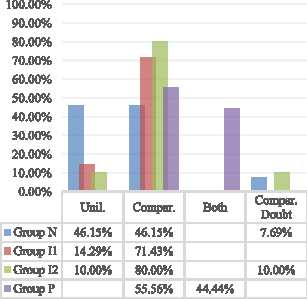
\includegraphics[width=.4\textwidth]{figures/quinci/figure5.pdf}
 \caption{Types of self-revision in relation to the ST in task 1 (percentage of participants per group)}
 \label{quinci:fig:5}
\end{figure}

\begin{figure}
 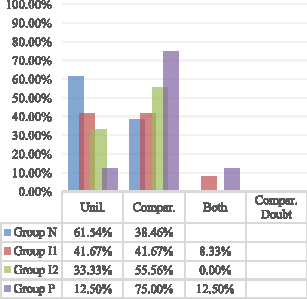
\includegraphics[width=.4\textwidth]{figures/quinci/figure6.pdf}
 \caption{Types of self-revision in relation to the ST in task 5 (percentage of participants per group)}
 \label{quinci:fig:6}
\end{figure}

Conversely, the data on the type of self-\isi{revision} carried out do show clear patterns. As is apparent from \figref{quinci:fig:5} and \figref{quinci:fig:6} above, the supposed level of TC seems to considerably affect the translators' approach to \isi{revision}. None of the professionals relied on simple unilingual self-\isi{revision} whereas \isi{novices} tended not to compare the TT and ST and seldom carried out both unilingual and comparative self-\isi{revision}. Data highlight a rather consistent shift from unilingual to comparative self-\isi{revision} in (more) experienced translators, with unilingual self-\isi{revision} being the preferred option for \isi{novices} and first-year intermediates in four out of five tasks. Conversely, second-year intermediates and professionals mostly relied on comparative self-\isi{revision}, which is the most-chosen option in four tasks out of five for Group I\textsubscript{2} and in all tasks for Group P. Also, professionals are the only group which carried out both unilingual and comparative self-\isi{revision} in all tasks, though with a decreasing percentage of participants throughout the five tasks.


These trends once again suggest self-confidence in less experienced translators, who do not seem aware that their translations might need careful self-\isi{revision}. As pointed out by \citet[439]{TirkkonenCondit1992}, ``[t]he professional is more modest, and more sensitized to noticing those areas in her translation that may need checking. The non-professional, in contrast, seems to be more arrogant in her approach and does not voice a need to have her translation checked''.


Moreover, as reported by \citet{Mossop2007Empirical}, \citet{Brunette2005} found that ``comparative \isi{revision} [yields] a better quality final product than unilingual, not only (as one might expect) with regard to accuracy but also with regard to the readability, the linguistic correctness and the appropriateness to purpose and to readership of the revised translations''. Such an inattentive and rather superficial approach to the final phase of the \isi{translation process} might thus considerably affect \isi{translation quality}, which is presumed to improve following more accurate checking.


\section{Process-related data and translation acceptability}

The research design of the empirical study also involved the quality assessment of the TTs produced by the sample, with the aim to find possible correlations between the supposed levels of TC of the participants, the textual and procedural patterns identified and \isi{translation quality}, which was assessed in terms of both translation \isi{acceptability} and translation error analysis. Given the considerable number of TTs produced (239) and the need for experienced external evaluators who could assess all the translations in order to ensure consistent assessment, the best option for evaluating translation \isi{acceptability} was the use of the experimentally verified \citep{Castillo2010} method devised by PACTE based on the so-called ``rich points''
(\citealt{PACTE2005Primeros}, \citealt{PACTE2009}). This method involves the identification of specific textual elements in the ST, i.e. rich points (RPs) which ``provide variety in the types of translation problems studied, [and] do not lead to immediate and acceptable solutions'' \citep[614]{PACTE2005Investigating}. Such RPs, which in this study have been identified by several participants from each group, have been evaluated as `acceptable', `partially acceptable' or `unacceptable' by three translator trainers on the basis of the criteria identified by \citet[217]{PACTE2009}, so as to obtain a numeric `\isi{acceptability} index' (AI). Based on their AIs -- ranging from 0 to 9, as the number of RPs identified in each ST --, participants were divided in five different performance levels: Level I (0-1.9); Level II (2-3.9); Level III (4-5.9); Level IV (6-7.9); Level V (8-9).

The ranking of the average AIs in \figref{quinci:fig:7} below shows that professionals are the outperforming group in three out of five tasks and recorded the second highest AI in tasks 1 and 3.

\begin{figure}
 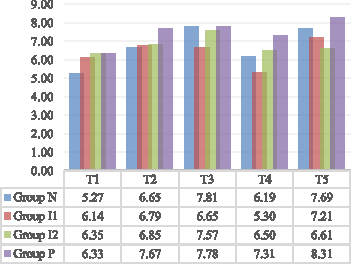
\includegraphics[width=.4\textwidth]{figures/quinci/figure7.pdf}
 \caption{Average acceptability index per group}
 \label{quinci:fig:7}
\end{figure}

On the other hand, \isi{novices} do not hold a stable position in the ranking, scoring the lowest AIs in tasks 1 and 2, the second and third highest indexes in tasks 4 and 5 respectively, and the highest AI in task 3. Similarly, second-year intermediates fluctuate between the highest and the lowest position, whereas first-year intermediates consistently scored the (second) lowest AIs in all tasks. It should be noted that Groups I\textsubscript{1} and I\textsubscript{2} scoring lowest in the last three tasks correspond to the same cohort (Ic), which consistently recorded the lowest AIs in all the three tasks carried out, with about 50\% of its participants scoring low to medium AIs (between 4 and 5.5).\footnote{This does not imply that (all) trainees in cohort Ic have not developed their TC at all, but only that their AIs were \textit{on} \textit{average} lower as compared to those scored by the other groups. It should also be considered that students with different backgrounds and coming from different universities and degree programmes can enrol in the MA programme who might lack a proper training in translation. However, despite the presence of some consistently underperforming participants in cohort Ic, there was a general tendency for the whole cohort to score lower values, possibly because it simply comprised less trained, less motivated and/or less skilled translators.} This might of course affect the analysis based on the final ranking shown in \figref{quinci:fig:7}, which thus needs to be supported by data on the distribution of the participants within the five abovementioned performance levels. The analysis considers the percentage of participants per group falling within each performance level (\tabref{quinci:tab:6}).

\begin{table}
 \caption{Distribution of the participants within the performance levels in task 3}
 \label{quinci:tab:6}
\begin{tabularx}{\textwidth}{XXXXX}
\lsptoprule
\multicolumn{1}{X}{Task 3} & \multicolumn{1}{X}{N} & \multicolumn{1}{X}{ I\textsubscript{1}} & \multicolumn{1}{X}{I\textsubscript{2}} & \multicolumn{1}{X}{P}\\
\midrule
PL I (0-1.9) &  &  &  & \\
PL II (2-3.9) &  &  &  & \\
PL III (4-5.9) & 15.38\% & 40.00\% &  & \\
PL IV (6-7.9) & 38.46\% & 30.00\% & 71.42\% & 55.55\%\\
PL V (8-9) & 46.15\% & 30.00\% & 28.57\% & 44.44\%\\
\lspbottomrule
\end{tabularx}
\end{table}

\tabref{quinci:tab:6} above shows the internal distribution of the four groups in task 3, where \isi{novices} scored the highest AI, followed by professionals and second- and first-year intermediates, respectively (see \figref{quinci:fig:7}). Despite their highest AI, however, only 84.61\% of \isi{novices} fell within the two highest levels of performance (i.e. levels IV and V) as compared to 100\% of both second-year intermediates and professionals. As in other tasks -- the results of which are not reported here in detail for reasons of space -- \isi{novices}' scores tend to cover a wider range of AIs (i.e. 5.5-9 in the third task) as compared to groups I\textsubscript{2} and P (i.e. 6.5-8 and 6.5-9 respectively in task 3), which means that more experienced translators tend to produce on average medium- to high-quality TTs, whereas \isi{novices} include both out- and underperforming participants.

Hence, it could be concluded that professionals generally show a ``consistently superior performance'' \citep[215]{Jaaskelainen2010} as compared to less experienced translators, whose performances tend to spread across more performance levels.

\section{Data triangulation: Painting the global picture}

The comparative analysis of the variables examined in the previous sections suggests that \isi{novices}' comparatively lower delivery time and higher self-assessment scores do not result from an underestimation of the difficulty of the task to be performed. The almost consistent inverse proportion between self-assessment scores and average perceived text difficulty showed that all groups can assess the difficulty of the tasks and rank them accordingly. Hence, it seems that the development of TC and the self-\isi{perception} of the quality of the performance are somehow related and that such relation may be represented as a parabola opening upwards -- where TC is a continuum on the horizontal axis -- with \isi{novices} and professionals corresponding to the two ends of the branches and intermediates to the vertex in the lower part of the curve. This trend undoubtedly highlights a high level of self-confidence in \isi{novices}, who seem unaware of their actual level of TC and/or the parameters for assessing \isi{translation quality}.

Data on translation \isi{acceptability} and self-\isi{revision} seem to confirm this hypothesis since \isi{novices}' consistently high self-assessment scores do not always parallel high \isi{acceptability} indexes. Also, \isi{novices} tend to score lower AIs and distribute more heterogeneously among the five performance levels identified as compared to more experienced translators. In addition, \isi{novices} seem to be the least careful revisers in the sample, as they tend to rely solely on unilingual self-\isi{revision}, which does not allow for the easy detection of potential inaccuracies and omissions, as opposed to professionals who mostly performed comparative self-\isi{revision}, followed in some cases by unilingual re-reading. Hence, the significant self-confidence displayed by \isi{novices} appears unjustified and (at least partially) misplaced. 

\newpage 
Their inexperience also emerges from the analysis of the number and type of different materials used, indicating that professionals generally needed a more restricted variety of reference materials and mainly used mono- and bilingual dictionaries, as opposed to students who also heavily relied on on-line search engines. This might suggest that, given that the STs were non-specialist articles dealing with well-known topics, professionals' wider FLS \citep[47]{Bell1991} allowed them to translate more effortlessly and quickly -- and ultimately with better results as concerns translation \isi{acceptability}.

The results of this analysis have been used to develop a model of TC describing the trends observed within the different stages identified in the development of TC \citep{Quinci2015b}. In this model (\figref{quinci:fig:8}),\footnote{This is an abridged version of the original model, where other trends relating to the additional variables investigated within PhD research project are also included (cf. \citealt{Quinci2015b}; available at \url{http://hdl.handle.net/10077/10986}).} TC is represented as a continuum extending from the initial stage of `novice' to that of `professional/competent' translator, thus describing the progressive evolution of the trends from one stage to the other.

\begin{figure}
    \resizebox{\textwidth}{!}{
    \begin{tikzpicture}
        \usetikzlibrary{positioning}
        % Define Styles
        \tikzstyle{block} = [
            rectangle, 
            fill=white, 
            align = center,
            minimum height=10em, 
            minimum width = 15em, 
            font = \sffamily
        ]
        % Place nodes
        \node [
            block, 
            fill=lsMidOrange!20,
            draw = lsMidOrange!20
        ] (A) {%
            \textbf{Novice}\\ \\
            Unawareness\\
            Overconfidence\\ 
            Lack of \isi{self-monitoring} skills\\
            Lack of time-management skills
        };    
        \node [
            block, 
            right = 3em of A, 
            fill=lsMidOrange!40,
            draw=lsMidOrange!40
        ] (B) {%
            \textbf{Intermediate}\\ \\
            Limited self-\isi{perception}\\
            Lack of self-confidence\\
            Greater \isi{self-monitoring} skills\\
            Greater focus on accuracy 
        };
        \node [
            block, 
            right = 3em of B, 
            fill=lsMidOrange!60,
            draw=lsMidOrange!60
        ] (C) {%
            \textbf{Professional}\\ \\
            Self-awareness\\
            Self-monitoring skills\\
            More extended FLS\\
            Focus on accuracy and meaning 
        };
        % Fill triangles
        \fill[fill=lsMidOrange!20] (A.north east) -- (B.west) -- (A.south east) -- cycle;
        \fill[fill=lsMidOrange!40] (B.north east) -- (C.west) -- (B.south east) -- cycle;
        \fill[fill=lsMidOrange!40] (B.north west) -- (A.north east) -- (B.west) -- cycle;
        \fill[fill=lsMidOrange!40] (B.south west) -- (A.south east) -- (B.west) -- cycle;
        \fill[fill=lsMidOrange!60] (C.north west) -- (B.north east) -- (C.west) -- cycle;
        \fill[fill=lsMidOrange!60] (C.south west) -- (B.south east) -- (C.west) -- cycle;
    \end{tikzpicture}
    }
    \caption{The trends observed within the three stages of TC}
    \label{quinci:fig:8}
\end{figure}

In the first stages of their training, inexperienced (and necessarily) incompetent trainees tend to be overconfident and openly unaware of their lacking experience and competence in translation. This emerges from their superficial and simplistic approach to \isi{revision}, which is often combined with low delivery time and high self-assessment. The trends observed in intermediate participants show instead that they have developed a greater awareness of their abilities and limits. They generally spent the longest time on the task and gradually shifted from unilingual to comparative self-\isi{revision}. In spite of this, their consistently lower self-assessment scores as compared to \isi{novices} testify to a general lack of self-confidence, probably combined with a greater awareness of the quality standards required of professional translators. This appears to be confirmed by the fact that intermediates tend to perform comparative (vs. unilingual) self-\isi{revision} and ultimately reach higher levels of accuracy than \isi{novices}. Finally, professionals appeared to be fully aware of their competence and display a level of self-confidence that is proportional to the quality of their performance.

Another key feature of increasing TC is the development of time-management skills, which in turn lead to higher efficiency. Novices tend to be faster than intermediates but evidently do not use the time at their disposal to improve the quality of their work, as suggested by the data on self-\isi{revision}, as opposed to professionals, who are the group placing the greatest focus on accuracy and meaning. Apparently, their more extended FLS and FSS (``Frequent Lexis Store'' and ``Frequent Structure Store'', \citealt{Bell1991}) allow them to select equivalents faster than trainees and to focus on \isi{revision} and accuracy, which ultimately increased the quality of their performance.

\section{Concluding remarks}

This paper has presented a longitudinal analysis of some process- and product-related data highlighting features of self-confidence and unawareness in novice vs. more experienced translators. Data have been collected within an empirical longitudinal study carried out at the University of Trieste with the aim to investigate TC and its development through a combined approach, which is primarily product-oriented but also included process-related data. The analysis outlined in the previous sections focused on the trends observed in the sample concerning the participants' delivery time and self-assessment, the perceived difficulty of the tasks performed, the reference materials used and the \isi{revision} phase of the \isi{translation process}, as well as translation \isi{acceptability}.

The contrastive analysis of less and more experienced and competent translators has highlighted the fundamental of training and experience by showing how these contribute to the development of \isi{self-monitoring} skills and affect self-\isi{perception}, in that they foster awareness in trainees of their still lacking competence and ultimately promote more careful \isi{revision} and rigorous self-assessment.

The above findings might be of great help in translator training to raise awareness in trainees about the possible consequences of overconfidence, particularly when it is not supported by actual competence. From a pragmatic point of view, trainees might ultimately come to realise that they are still largely inexperienced (and thus in need of appropriate training) and that their inexperience needs to be -- at least tentatively -- compensated by careful \isi{revising} and re-reading, which does not only improve the overall quality of their work, but also involves self-training and may encourage self-reflection on one's strengths and weaknesses.

\sloppy
\printbibliography[heading=subbibliography,notkeyword=this]
\end{document}

% \textbf{References}
% 
% \begin{styleNormalWeb}
% Bell, Roger T. 1991. \textit{Translation and Translating. Theory and Practice}. London and New York: Longman.
% \end{styleNormalWeb}
% 
% \begin{styleNormalWeb}
% Brunette, Louise, Chantal Gagnon, and Jonathan Hine. 2005. ``The GREVIS Project: Revise or Court Calamity.'' \textit{Across Languages and Cultures} 6(1):29--45.
% \end{styleNormalWeb}
% 
% \begin{styleNormalWeb}
% Castillo Rincón, Luis Miguel. 2010. ``La Evaluación de La Aceptabilidad de Las Traducciones. Un Estudio Exploratorio Sobre La Idoneidad de Los Puntos Ricos Para Evaluar Traducciones.'' Universitat Autónoma de Barcelona.
% \end{styleNormalWeb}
% 
% \begin{styleNormalWeb}
% Englund Dimitrova, Birgitta. 2005. \textit{Expertise and Explicitation in the Translation Process}. Amsterdam/Philadelphia: John Benjamins.
% \end{styleNormalWeb}
% 
% \begin{styleNormalWeb}
% Göpferich, Susanne. 2009. ``Towards a Model of Translation Competence and Its Acquisition: The Longitudinal Study TransComp.'' Pp. 11--37 in \textit{Behind the Mind: Methods, Models and Results in Translation Process Research}, vol. 03, edited by Susanne Göpferich, Arnt Lykke Jakobsen, and Inger M. Mess. Copenhagen: Samfundslitteratur.
% \end{styleNormalWeb}
% 
% \begin{styleNormalWeb}
% Hurtado Albir, Amparo, and Fabio Alves. 2009. ``Translation as a Cognitive Activity.'' Pp. 63--73 in \textit{The Routledge Companion to Translation Studies}, edited by Jeremy Munday. London \& New York: Routledge.
% \end{styleNormalWeb}
% 
% \begin{styleNormalWeb}
% Jääskeläinen, Riitta. 1996. ``Hard Work Will Bear Beautiful Fruit. A Comparison of Two Think-Aloud Protocol Studies.'' \textit{Meta: Journal des traducteurs} 41(1):60--74.
% \end{styleNormalWeb}
% 
% \begin{styleNormalWeb}
% Jääskeläinen, Riitta. 2010. ``Are All Professional Experts? Definitions of Expertise and Reinterpretation of Research Evidence in Process Studies.'' Pp. 213--27 in \textit{Translation and Cognition}, edited by Gregory M. Shreve and Erik Angelone. Amsterdam/Philadelphia: John Benjamins.
% \end{styleNormalWeb}
% 
% \begin{styleNormalWeb}
% Jensen, Astrid. 1999. ``Time Pressure in Translation.'' Pp. 103--20 in \textit{Probing the Process In Translation: Methods and Results}, edited by Gyde Hansen. Samfundslitteratur.
% \end{styleNormalWeb}
% 
% \begin{styleNormalWeb}
% Kiraly, Donald. 1995. \textit{Pathways to Translation: Pedagogy and Process}, Kent State University Press. 
%
% Kiraly, Don. 2013. ``Towards a View of Translator Competence as an Emerging Phenomenon.'' in \textit{New Prospects and Perspectives for Educating Language Mediators}, edited by D. Kiraly, K. Hansen-Schirra and S. Maksymski, Tübingen: Narr Verlag.
% 
% \begin{styleNormalWeb}
% Krings, Hans Peter. 1986. \textit{Was in Den Köpfen von Übersetzern Vorgeht: Eine Empirische Untersuchung Zur Struktur Des Übersetzungsprozesses an Fortgeschrittenen Französischlernern}.
% \end{styleNormalWeb}
% 
% \begin{styleNormalWeb}
% Kussmaul, Paul. 1995. \textit{Training the Translator}, Amsterdam/Philadelphia: John Benjamins.
%
% \begin{styleNormalWeb}
% Künzli, Alexander. 2001. ``Experts vs. Novices: L'utilisation de Sources D'information Pendant Le Processus de Traduction.'' \textit{Meta} 46(3):507--23. 
% \end{styleNormalWeb}
% 
% \begin{styleNormalWeb}
% Lesznyák, Márta. 2008. ``Studies in the Development of Translation Competence.''
% \end{styleNormalWeb}
% 
% \begin{styleNormalWeb}
% Lörscher, Wolfgang. 2012. ``Bilingualism and Translation Competence.'' \textit{SYNAPS - A Journal of Professional Communication} (27):3--15.
% \end{styleNormalWeb}
% 
% \begin{styleNormalWeb}
% Massey, Gary, and Maureen Ehrensberger-Dow. 2011. ``Investigating Information Literacy: A Growing Priority in Translation Studies.'' \textit{Across Languages and Cultures} 12(2):193--211.
% \end{styleNormalWeb}
% 
% \begin{styleNormalWeb}
% Mossop, Brian. 2007. ``Empirical Studies of Revision: What We Know and Need to Know.'' \textit{JosTrans. The Journal of Specialised Translation} (8):5--20.
% \end{styleNormalWeb}
% 
% \begin{styleNormalWeb}
% Mossop, Brian. 2014. \textit{Revising and Editing for Translators}. 3rd edition. Manchester: St. Jerome.
% \end{styleNormalWeb}
% 
% \begin{styleNormalWeb}
% Orozco, Mariana, and Amparo Hurtado Albir. 2002. ``Measuring Translation Competence Acquisition.'' \textit{Meta} 47(3):375--402.
% \end{styleNormalWeb}
% 
% \begin{styleNormalWeb}
% PACTE. 2002. ``Exploratory Tests in a Study of Translation Competence.'' \textit{Conference Interpretation and Translation} 4(2):41--69.
% \end{styleNormalWeb}
% 
% \begin{styleNormalWeb}
% PACTE. 2003. ``Building a Translation Competence Model.'' Pp. 43--66 in \textit{Triangulating Translation: Perspectives in Process-Oriented Research}, edited by Fabio Alves. Amsterdam/Philadelphia: John Benjamins.
% \end{styleNormalWeb}
% 
% \begin{styleNormalWeb}
% PACTE. 2005a. ``Investigating Translation Competence: Conceptual and Methodological Issues.'' \textit{Meta} 50(2):609--19.
% \end{styleNormalWeb}
% 
% \begin{styleNormalWeb}
% PACTE. 2005b. ``Primeros Resultados de Un Experimento Sobre La Competencia Traductora.'' Pp. 573--87 in \textit{Actas del II Congreso Internacional de la AIETI (Asociación Ibérica de Estudios de Traducción e Interpretación) ``Información y documentación.''}Madrid: Publicaciones de la Universidad Pontificia Comillas.
% \end{styleNormalWeb}
% 
% \begin{styleNormalWeb}
% PACTE. 2009. ``Results of the Validation of the PACTE Translation Competence Model: Acceptability and Decision Making.'' \textit{Across Languages and Cultures} 10(2):207--30.
% \end{styleNormalWeb}
% 
% \begin{styleNormalWeb}
% Quinci, Carla. 2015a. ``Defining and Developing Translation Competence for Didactic Purposes: Some Insights from Product-Oriented Research.'' in \textit{Handbook of Research on Teaching Methods in Language Translation and Interpretation}, edited by Ying Cui and Wei Zhao. IGI Global.
% \end{styleNormalWeb}
% 
% Quinci, Carla. 2015b. \textit{Translators in the Making: An Empirical Longitudinal Study on Translation Competence and its Development}. PhD dissertation, Università degli Studi di Trieste. Available at \url{http://hdl.handle.net/10077/10986}.
% 
% \begin{styleNormalWeb}
% Ronowicz, Eddie, Joanna Hehir, Toshihiro Kaimi, Keiko Kojima, and Deok-Shin Lee. 2005. ``Translator's Frequent Lexis Store and Dictionary Use as Factors in SLT Comprehension and Translation Speed -- A Comparative Study of Professional, Paraprofessional and Novice Translators.'' \textit{Meta: Journal des traducteurs} 50(2):580--96.
% \end{styleNormalWeb}
% 
% \begin{styleNormalWeb}
% Shreve, Gregory M. 1997. ``Cognition and the Evaluation of Translation Competence.'' Pp. 233--51 in \textit{Cognitive Processes in Translation and Interpreting}, edited by J. H. Danks, Gregory M. Shreve, S. B. Fountain, and M. K. McBeath. London: Sage.
% \end{styleNormalWeb}
% 
% \begin{styleNormalWeb}
% Tirkkonen-Condit, Sonja. 1992. ``The Interaction of World Knowledge and Linguistic Knowledge in the Processes of Translation: A Think-Aloud Protocol Study.'' Pp. 433--40 in \textit{Translation and Meaning. Proceedings of the Łódź Session of the 1990 Maastricht-Łódź Duo Colloquium on Translation and Meaning}, edited by B. Lewandowska-Tomaszczyk and M. Thelen. Maastricht: Faculty of Translation and Interpreting.
% \end{styleNormalWeb}
